\documentclass[12pt,letterpaper]{article}
\usepackage[latin1]{inputenc}
\usepackage[spanish]{babel}
\usepackage{graphicx}
\usepackage[left=2cm,right=2cm,top=2cm,bottom=2cm]{geometry}
\usepackage{graphicx} % figuras
\usepackage{subfigure} % subfiguras
\usepackage{float} % para usar [H]
\usepackage{amsmath}
\usepackage{txfonts}
\usepackage{stackrel} 
\usepackage[latin1]{inputenc}
\usepackage{multirow}
\usepackage{enumerate} % enumerados
\renewcommand{\labelitemi}{$-$}
\renewcommand{\labelitemii}{$\cdot$}
\author{Fanny Clemente}
\title{Caratula}
\begin{document}



\author{Fanny Clemente}
\title{Caratula}

\begin{titlepage}
\begin{center}
\large{UNERSIDAD PRIVADA DE TACNA}\\
\vspace*{-0.025in}
\begin{figure}[htb]
\begin{center}

\includegraphics[width=8cm]{./IMG/logo}
\end{center}
\end{figure}
\vspace*{0.15in}
INGENIERIA DE SISTEMAS  \\

\vspace*{0.5in}
\begin{large}
TITULO:\\
\end{large}

\vspace*{0.1in}
\begin{Large}
\textbf{Instalacion de Base de Datos Oracle} \\
\end{Large}

\vspace*{0.3in}
\begin{Large}
\textbf{CURSO:} \\
\end{Large}

\vspace*{0.1in}
\begin{large}
BASE DE DATOS II\\
\end{large}

\vspace*{0.3in}
\begin{Large}
\textbf{DOCENTE(ING):} \\
\end{Large}

\vspace*{0.1in}
\begin{large}
 Patrick Cuadros Quiroga\\
\end{large}

\vspace*{0.2in}
\vspace*{0.1in}
\begin{large}
Integrantes: \\
\begin{flushleft}
Acevedo Vásquez, Leonardo Fernando 	(2014047512) \\
Andía Bernedo, Josei Jomar 			(2014049093) \\
Condori Velarde, Sonia          	(2014049546) \\
Clemente Cruz, Fanny Luz    		(2014049550) \\
Flores Colque, Gisela           	(2014049547) \\
Llatasi Cohaila, Cristian Omar		(2014037546) \\
Morales Anquise, Tommy Edwards 		(2015050480) \\
Ticona Arcaya, Sergio Alexis		(2014049171) \\
Tapia Ticona, Lupe Carolina			(2014049548) \\
\end{flushleft}
\end{large}
\end{center}

\end{titlepage}




 \tableofcontents
 \newpage
SESI0N DE LABORATORIO N° 07:
Instalacion de Oracle Database 12c
 
\section{INTRODUCCION} 
 \newpage
\section{Objetivos} 
\newpage
\section{Oracle Linux modo Terminal}
\subsection{Instalacion}


\subsection{implementacion}

\subsection{Configuracion}


\newpage

\section{Windows Server}
\subsection{Instalacion}
Primero descargar el fichero ejecutable desde la página principal de Oracle.
Después de descargar el fichero, descomprimir la carpeta que lo contiene,
posteriormente, ubicar el archivo en donde se encuentra el ejecutable y
hacer doble clic en el setup.
\begin{center}
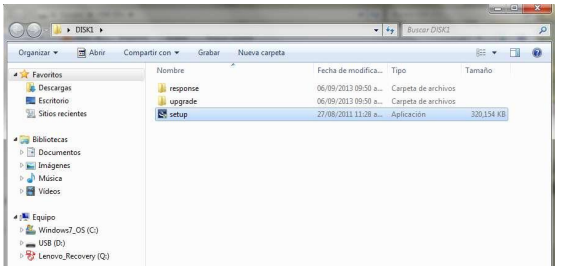
\includegraphics[width=15cm]{./IMG/img1}
\end{center} 
Posteriormente ejecutar esta aplicacion y aceptar los permisos aparecera el
instalador del gestor de base de datos.
\begin{center}
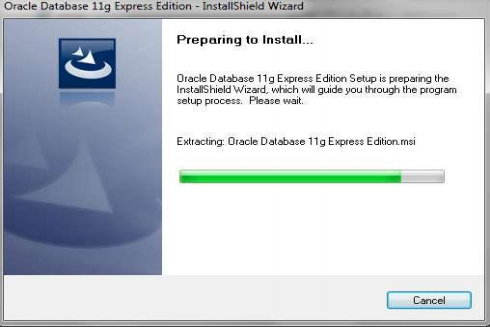
\includegraphics[width=15cm]{./IMG/img2}
\end{center} 
Ahora procedemos a instalarlo y el asistente empezará dicho proceso
\begin{center}
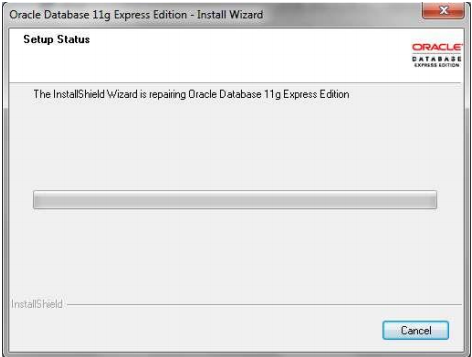
\includegraphics[width=15cm]{./IMG/img3}
\end{center} 


A continuacion nos pedira el nombre de usuario y una contrasena, estas deberán
ser ingresadas por el Administrador de la base de datos, con esto ingresaremos al
Sistema Gestor de Base de Datos. Finalmente cuando el asistente finaliza con la
instalacion iniciaremos la base de datos:\\
Para esto deberá ir al menú inicio de Windows, clic en todos los programas,
localiza Oracle Database 11g Express Edition y después en Get Sarted
\begin{center}
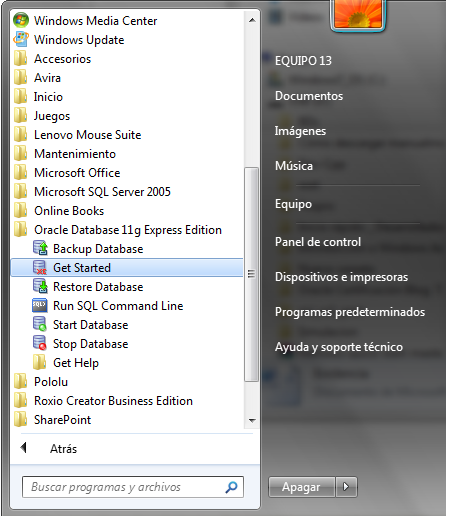
\includegraphics[width=15cm]{./IMG/img4}
\end{center} 
Ahora iniciará el gestor de Base de Datos, se mostrará la pantalla de inicio
\begin{center}
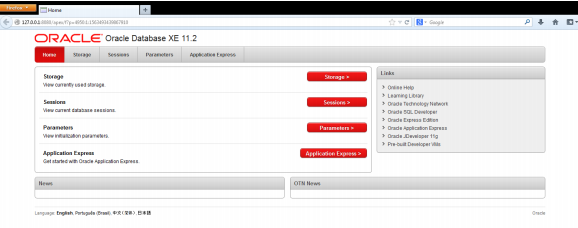
\includegraphics[width=15cm]{./IMG/img5}
\end{center} 


\subsection{implementacion}
\subsubsection{ Creacion WorkSpace}

\textbf{Proposito}:\\
El alumno pondrá en práctica los conocimientos teorícos, crea un workspace (espacio
de trabajo) en Oracle, para posteriormente crear la base de datos dentro de dicho
sistema gestor de base de datos Oracle 11 g Edicion Express (XE, por sus siglas en
ingles), y se comprueba su funcionamiento.\\
\textbf{Alcances}:\\
Instalacion de Oracle Database 11g XE.
Comprobar su funcionamiento.\\
\textbf{Requerimientos:}:\\
Equipo de computo, red, internet.
Sistema operativo Windows o linux.
Oracle Database 11g XE.
Tiempo estimado: 2 horas.\\
\textbf{Desarrollo}:\\
iniciar el la base de datos
\begin{center}
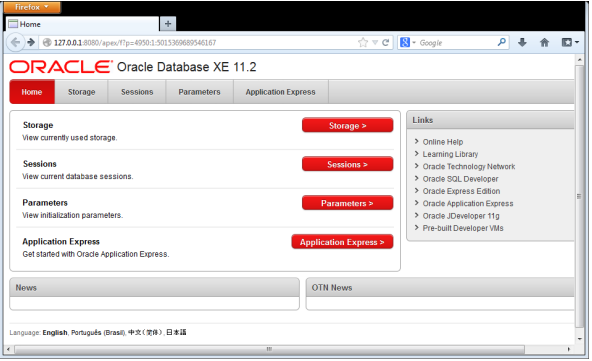
\includegraphics[width=15cm]{./IMG/img6}
\end{center}

Ir a Application Express, después validarnos como usuario. Ahora se procede a
crear un Workspace (figura 2.2), llenando el formulario, en donde ingresamos el
nombre de la base de datos, el nombre de usuario y por último la
contrasena para poder acceder:
\begin{center}
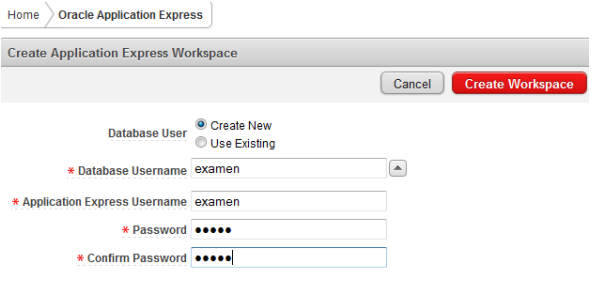
\includegraphics[width=15cm]{./IMG/img7}
\end{center}
Una vez creado muestra un mensaje de confirmacion, indicando que el
Workspace se ha creado correctamente. Posteriormente, se procede a acceder al
espacio de trabajo.
\begin{center}
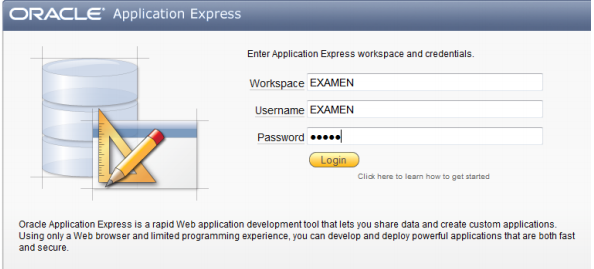
\includegraphics[width=15cm]{./IMG/img8}
\end{center}
Una vez ingresado se muestra la siguiente imagen
\begin{center}
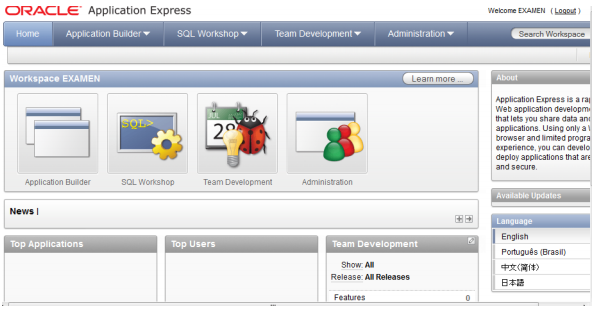
\includegraphics[width=15cm]{./IMG/img9}
\end{center}

\subsubsection{Creacion de Base de datos de Oracle}

\textbf{Proposito}:\\
Se realiza la creacion de la base de datos con gestor de base de datos Oracle 11 g
Edicion Express, y se comprueba su funcionamiento.\\
\textbf{Alcances}:\\
Creacion de base de datos denominada MIBASE 02 en Oracle Database
Comprobar su funcionamiento.\\
\textbf{Requerimientos:}:\\
Equipo de computo, red, internet.\\
Sistema operativo Windows o linux.\\
Oracle Database 11g XE.\\
Tiempo estimado: 2 horas\\
\textbf{Desarrollo}:\\
Una vez inicializado en gestor de base de datos selecciona la página principal del
WokrkSpace

\begin{center}
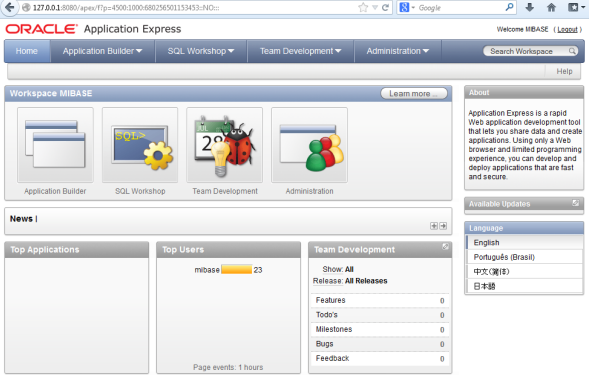
\includegraphics[width=15cm]{./IMG/img10}
\end{center}
Selecciona la solapa Appliction Buildes, posteriormente Database Applications,
pulsa clic en el boton Create. 
\begin{center}
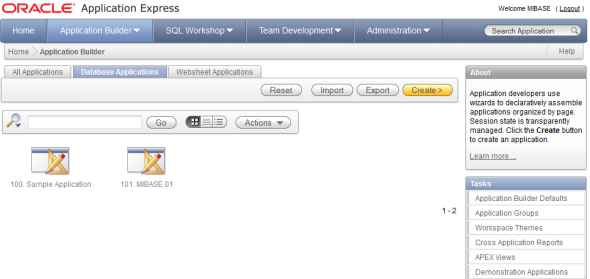
\includegraphics[width=15cm]{./IMG/img11}
\end{center}
Se pueden crear diferentes tipos de aplicaciones (Database, Websheet, Sample
Applications). Seleccionar el tipo database y da clic en siguiente.

\begin{center}
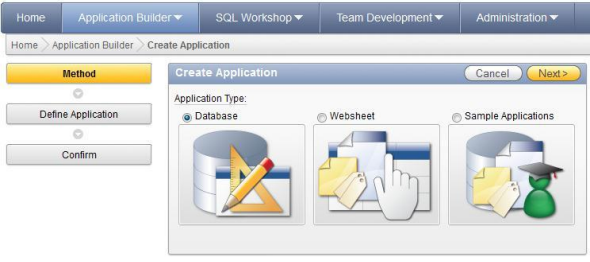
\includegraphics[width=15cm]{./IMG/img12}
\end{center}
Posteriormente deberas llenar todos los campos que requiere la BD (método,
esquema, id) y finalmente Confirmar

\begin{center}
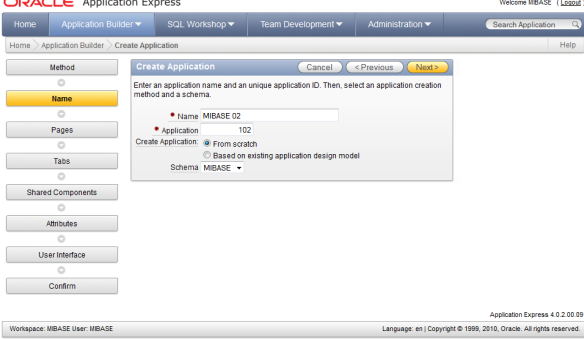
\includegraphics[width=15cm]{./IMG/img13}
\end{center}
\subsubsection{Creacion de Base de datos de Oracle}

\textbf{Proposito}:\\
Se realiza la creacion de entidades (tablas) asignadas a la base de datos que se
creo en la practica anterior con gestor de base de datos Oracle 11 g Edicion
Express, y se comprueba su funcionamiento.\\
\textbf{Alcances}:\\
Creacion de entidades en Oracle Database 11g XE.
Asignacion e identificacion diferentes tipos de de datos para los atributos, haciendo
uso del diccionario de datos del caso de estudio. \\
\textbf{Requerimientos:}:\\
Equipo de computo, red, internet.\\
Sistema operativo Windows o Linux.\\
Oracle Database 11g XE.\\
Tiempo estimado: 2 horas.\\
\textbf{Desarrollo}:\\
Una vez inicializado el gestor de base de datos selecciona la página principal del
WokrkSpace. Da clic en la solapa Appliction Buildes, posteriormente Database
Applications. Ahí encontraras las bases de datos que hayas creado. p.e la figura
4.1 muestra la BDs (101 MIBASE 01). Seleccione y pulse doble clic sobre el
icono.

\begin{center}
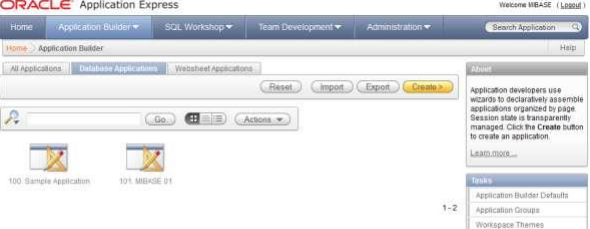
\includegraphics[width=15cm]{./IMG/img14}
\end{center}
Una vez hecha la seleccion podras observar el menu como lo muestra la figura
4.2. En la cual tendras dos opciones de menú gráfico y contextual, ambos servirán
para el manejo y administracion de la base de datos.
\begin{center}
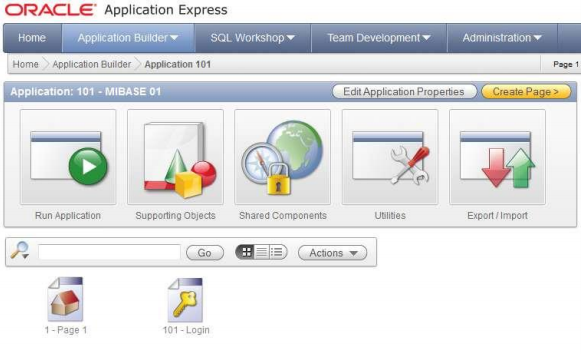
\includegraphics[width=15cm]{./IMG/img15}
\end{center}
Posteriormente selecciona la solapa del menú contextual de la parte superior de la
pantalla denominado SQL Workshop, acontinuacion Object Browser. Finalmente
se vizualiza una pantalla que te indica en la parte lateral derecha de la patalla que
tipos de objetos puedes crear, p.e tablas (entidades), vistas, procesos, funciones,
por mencionar algunas.
\begin{center}
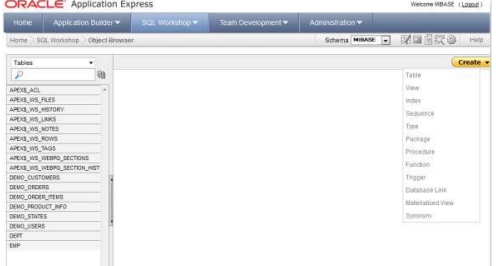
\includegraphics[width=15cm]{./IMG/img16}
\end{center}
Selecciona el tipo de objeto y da clic en el boton create (figura 3.4). Para este
caso selecciona Table, una vez hecha esta seleccion podras ingresar los campos
o atributos a la entidad, es decir asignar las columnas de la tabla, para ello es
necesario hacer uso del diccionario de datatos creado durante el diseno conceptual
y logico de la base de datos. 

\begin{center}
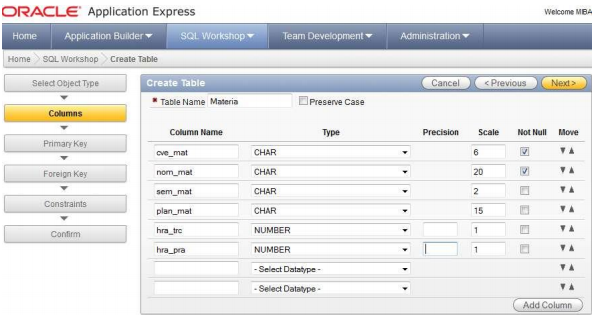
\includegraphics[width=15cm]{./IMG/img17}
\end{center}
Seleccionar la clave primaria y Next. 
\begin{center}
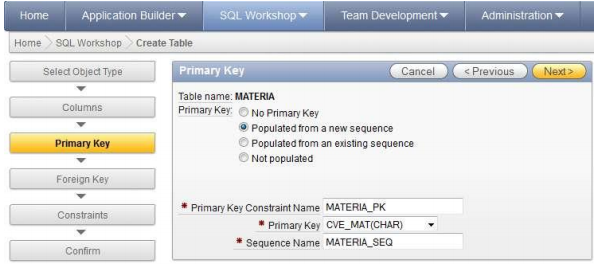
\includegraphics[width=15cm]{./IMG/img18}
\end{center}
Para este caso no existirá ninguna clave foránea y por lo tanto damos en
siguiente. Para las restricciones, no se hace nada y finalmente damos en créate
para crear nuestra tabla. 
\begin{center}
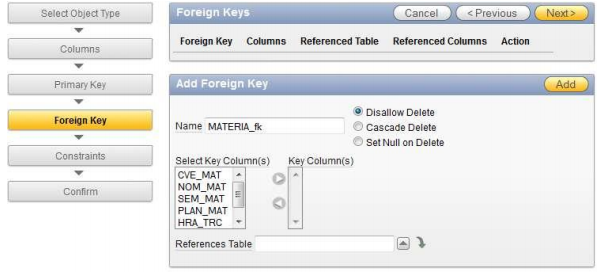
\includegraphics[width=15cm]{./IMG/img19}
\end{center}
Confirmacion de los datos con sentencias SQL de la tabla
\begin{center}
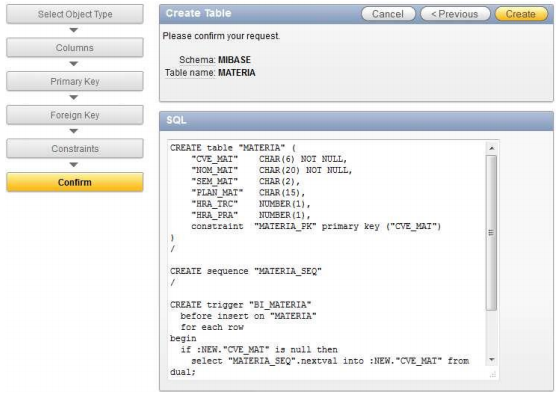
\includegraphics[width=15cm]{./IMG/img20}
\end{center}
Finalmente se puede visualizar la entidad Materia, aunado a esto podras observar
un menú contextual que te permite crear y administrar la entidad. 
\begin{center}
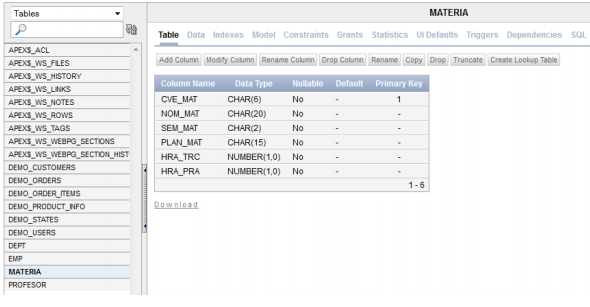
\includegraphics[width=15cm]{./IMG/img21}
\end{center}

Actividad extraclase: Ahora procede a crear las tablas: Teléfono,
MAT ANTERIOR, PROF PROFESION, PROFESION, EQUIVALENCIA, AULA,
GRUPO, HORARIO Y APRECIACION. Una vez terminado de crear las doce
tablas tendras la siguiente vista: (4.10) Para mas informacion consulta Anexos B y
C.

\begin{center}
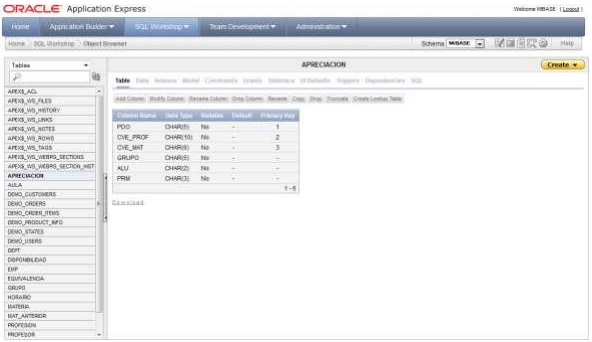
\includegraphics[width=15cm]{./IMG/img22}
\end{center}



\subsection{Configuracion}
 \newpage
 
 
 
\section{Solaris / Centos /BSD}
\subsection{Instalacion}
Antes de instalar cualquier SGBD es necesario conocer los requerimientos de hardware y software, el posible software a desinstalar previamente, verificar el registro de Windows y el entorno del sistema, así como otras caracteristicas de configuracion especializadas como pueden ser la reconfiguracion de los servicios TCP/IP y la modificacion de los tipos archivos HTML para los diversos navegadores.
Se presenta a continuacion una serie de requerimientos minimos de hardware y software para instalar Oracle Express 11g y MySQL estandar version 5.1. en y Ubuntu 14.
\begin{center}
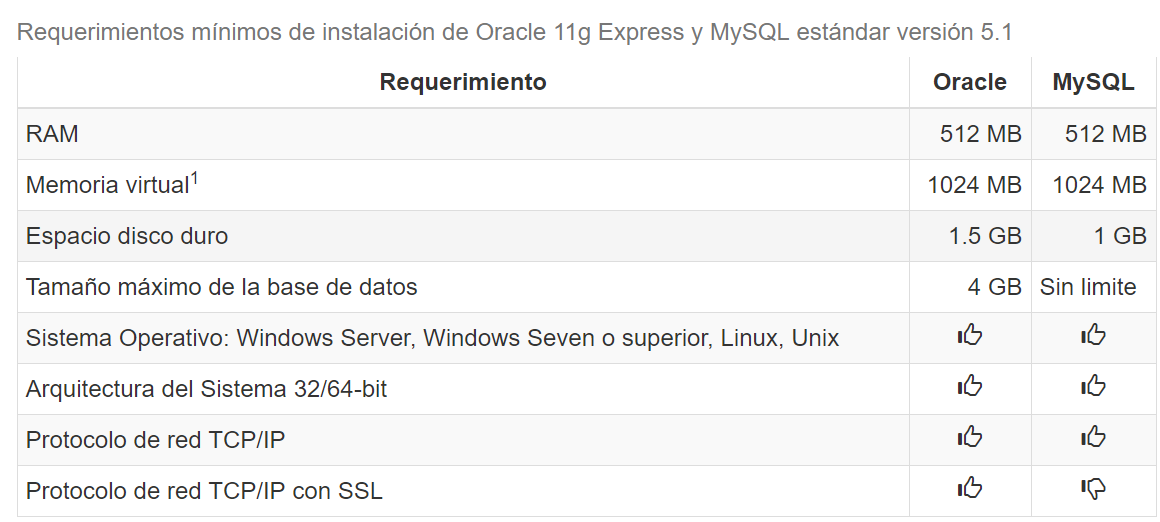
\includegraphics[width=15cm]{./IMG/img23}
\end{center}
\subsubsection{Proceso de instalacion}
Descarga el software apropiado a tu haradwawre y sistema operativo aqui\\
Descomprime el archivo descargado y ejecuta el archivo setup.exe (caso windows) con privilegios de administrador\\
Pulse sobre el boton de siguiente para iniciar la instalacion.\\
\begin{center}
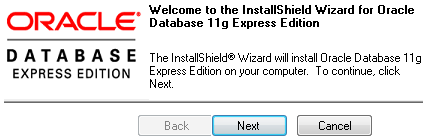
\includegraphics[width=15cm]{./IMG/img24}
\end{center}
Acepte los terminos de acuerdo de licencia
\begin{center}
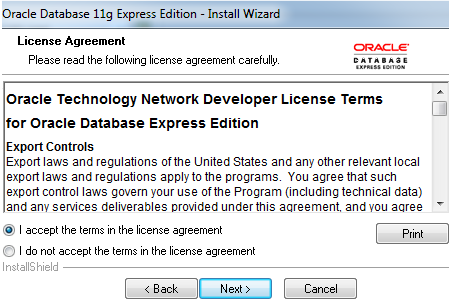
\includegraphics[width=15cm]{./IMG/img25}
\end{center}
Verifique los requerimientos de espacio y si los cumple pulse aceptar. Considere un Giga más para almacenamiento.
\begin{center}
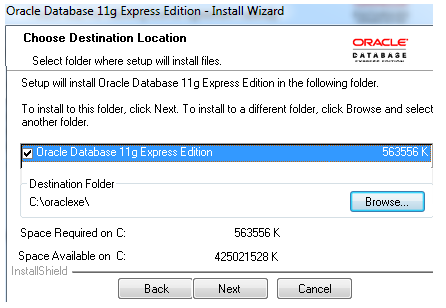
\includegraphics[width=15cm]{./IMG/img26}
\end{center}
Introduzca el password para el usuario SYSTEM. Despues de terminar la instalacion debera iniciar la base de datos con este usuario.

\begin{center}
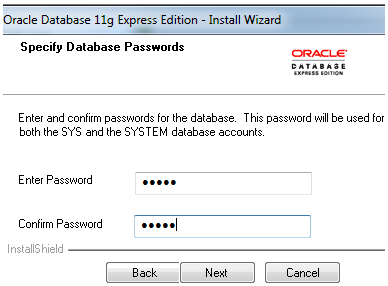
\includegraphics[width=15cm]{./IMG/img27}
\end{center}
A continuacion Oracle Database XE nos informa sobre los puertos que utilizara. Pulse Instalar.
\begin{center}
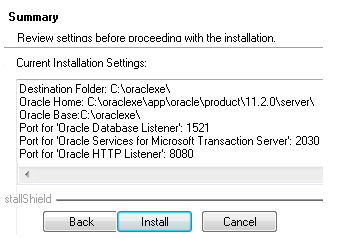
\includegraphics[width=15cm]{./IMG/img28}
\end{center}
El tiempo de instalacion de Oracle Database XE depende de su equipo (procesador y memoria). Al terminar el proceso de instalacion pulse el boton Terminar.
\begin{center}
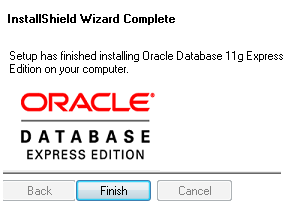
\includegraphics[width=15cm]{./IMG/img29}
\end{center}
Al pulsar el boton Terminar nos direccionara a la pagina de acceso de la base de datos (http://127.0.0.1:8080/apex). Recuerde iniciar por primera vez con el usuario SYSTEM y su password.
\begin{center}

\includegraphics[width=15cm]{./IMG/img30}
\end{center}
Pulse el icono Sessions e introduzca la siguiente informacion

\begin{center}
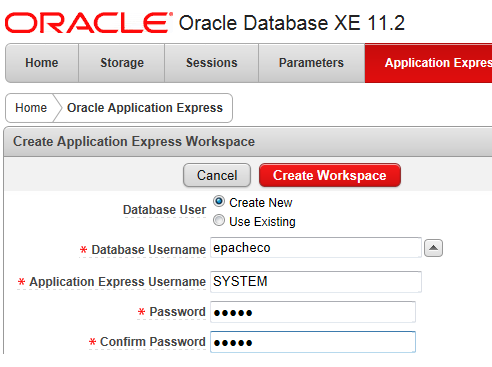
\includegraphics[width=15cm]{./IMG/img31}
\end{center}
Para futuros accesos usted puede pulsar boton de inicio, todos los programas, base de datos 11g Express Edition o el icono en su escritorio denominado Base de Datos.
\begin{center}
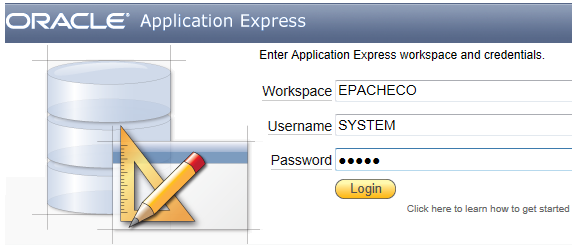
\includegraphics[width=15cm]{./IMG/img32}
\end{center}
Ahora vamos a crear un usuario
\begin{center}
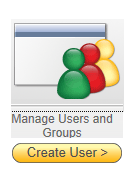
\includegraphics[width=8cm]{./IMG/img33}
\end{center}
llenar todo el formulario
\begin{center}
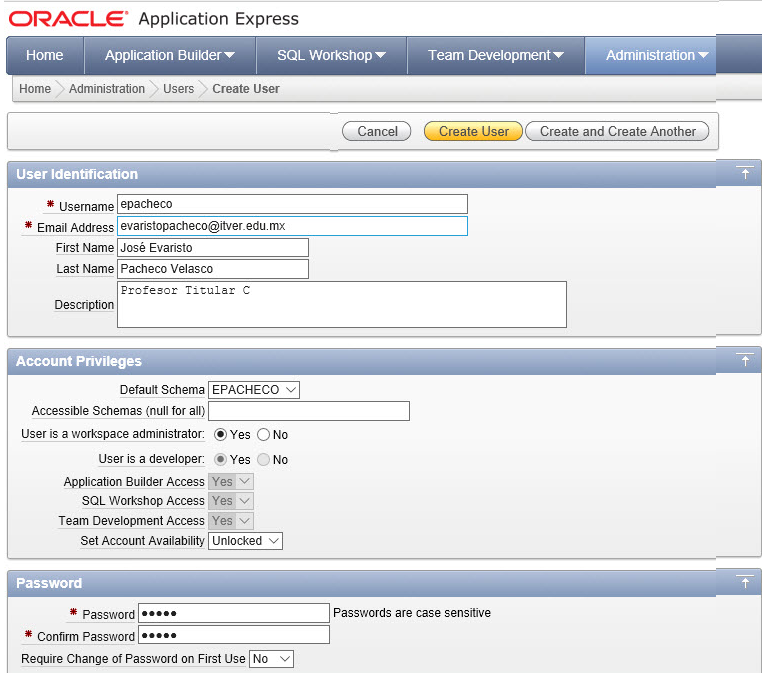
\includegraphics[width=15cm]{./IMG/img34}
\end{center}

\subsection{implementacion}
\subsection{Configuracion}





\section{WEBGRAFIA } 
- http://ri.uaemex.mx/bitstream/handle/20.500.11799/31602/secme-15942.pdf?sequence=1\\
- http://www.prograweb.com.mx/tallerBD/0101InstalarSGBD.php

\end{document}
